\documentclass[12p]{article}
\usepackage[margin=1in, headheight=110pt]{geometry}
\usepackage{amssymb, amsmath, amsfonts, amsthm}
\usepackage{mathpazo}
\usepackage{setspace}
\usepackage{fancyhdr}
\usepackage{hyperref}
\usepackage{float}
\usepackage{tikz}
\usepackage{enumitem}
\usepackage{graphicx}
\usepackage{listings}
\usepackage{caption}
\usepackage{bookmark}
\usepackage{multicol}

\newenvironment{hangingpar}[1]
  {\begin{list}
    {}
    {
      \setlength{\itemindent}{-#1}%%'
      \setlength{\leftmargin}{#1}%%'
      \setlength{\itemsep}{0pt}%%'
      \setlength{\parsep}{\parskip}%%'
      \setlength{\topsep}{\parskip}%%'
    }
    \setlength{\parindent}{-#1}%%
    \item[]
  }
  {\end{list}}

\def\ojoin{\setbox0=\hbox{$\bowtie$}%
  \rule[-.02ex]{.25em}{.4pt}\llap{\rule[\ht0]{.25em}{.4pt}}}
\def\leftouterjoin{\mathbin{\ojoin\mkern-5.8mu\bowtie}}
\def\rightouterjoin{\mathbin{\bowtie\mkern-5.8mu\ojoin}}
\def\fullouterjoin{\mathbin{\ojoin\mkern-5.8mu\bowtie\mkern-5.8mu\o}}

\pagestyle{fancy}
\lhead{Group Project Iteration 3 - Team 2}
\rhead{SENG 300 - Winter 2018}
\title{\vspace{-6ex}Group Project Iteration 2}
\date{\vspace{-12ex}}


\newcommand{\code}[1]{\texttt{#1}}

\setlength{\parindent}{3em}
\begin{document}
% \maketitle
\thispagestyle{fancy}

\begin{titlepage}
  \begin{center}
    \vspace{1cm}
    \Large{\textbf{University of Calgary}}\\
    \Large{\textbf{SENG 300  - Introduction to Software Engineering}}
    \vfill
    \line(1,0){400}\\[1mm]
    \huge{Group Project Iteration 3}\\
    \large{Anonymous, Local and Nested Types}\\
    \line(1,0){400}\\
    \Large April 9, 2018\\
    \vfill
    \huge{Team 2}\\
    \large
    \begin{multicols}{2}
      Evan Quan 10154242\\
      Marcello Di Benedetto 30031839\\
      Mona Agh 30033301\\
      John Benedict Bendoza 30028470\\
      Matthew Buhler 00332036\\
      Tyler Chow 30024575\\
      Dominic Demierre 300249784\\
      Philip Dometita 30032976\\
      Osagie Omigie 30008204\\
      Zheng Yang Toh 10129855\\
    \end{multicols}
  \end{center}
\end{titlepage}

\tableofcontents
\thispagestyle{empty}
\clearpage

\onehalfspacing

\setcounter{page}{1}

\section{Introduction}
This report details the use of a tool developed to parse java source code, 100 open source Java projects were selected to be analyzed to answer questions regarding nested, local, anonymous, and general Java declarations and references.
Over 150,000 declarations and 6 million references are included in this analysis.
From this data, the application of these declaration types were discussed for other Java and non-Java systems, and how their use may change across time.

\section{Data Collection and Results}
\subsection{Prevalence of Anonymous, Local, and Nested Type Declarations}


As shown in Figure \ref{fig:Declarations},  nested type declarations occupy about 20.53\% of the total number of declarations in the 100 systems. Averaging at 14.92\% with a median of 12.44\% per system. Both of these results have the outliers accounted for. In terms of the outliers, we managed to find two clear outliers: NullAway and JUnit4 which both have nested declarations almost four times higher than the average. Otherwise the number of nested declarations in each system are fairly equally distributed. This made it harder to spot outliers so we picked the two obvious outliers as to not skew the data.

\begin{figure}[h]
  \begin{center}
    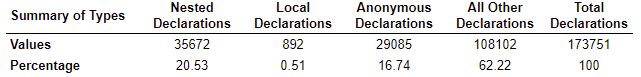
\includegraphics{Declarations.PNG}
    \caption{Total type declarations across all 100 Java systems}
    \label{fig:Declarations}
  \end{center}
\end{figure}

Local types are not declared much in almost all of the systems. Only 30\% of the systems in our sample have any local declarations, even within these systems, local declarations only make up around 1\% of the total declarations. Averaging 0.02\% with a median of 0\% per system when outliers are accounted for. There is one system that is composed of 34.51\% local declarations--690 times larger than the average--which is Dagger, a dependency injector for android and java. Otherwise, most of the outliers fall between 0.5\% to 2\% per system. From this we infer that local types are not widely used.

Anonymous classes are declared less than nested classes in our sample of 100 systems, accounting for 16.74\% of total declarations. But the average anonymous declaration per system is 19.57\% with a median of 15.09\% when outliers are accounted for. So when it comes to average usage, anonymous declarations are used more than nested declarations. This maybe due to anonymous classes being easier for casual use over nested classes. An anonymous class might be declared multiple times for overriding in one class while a nested class will be declared only once most of the time. Although some of the systems in our data seems to disagree with this notion.

\begin{figure}[H]
  \begin{center}
    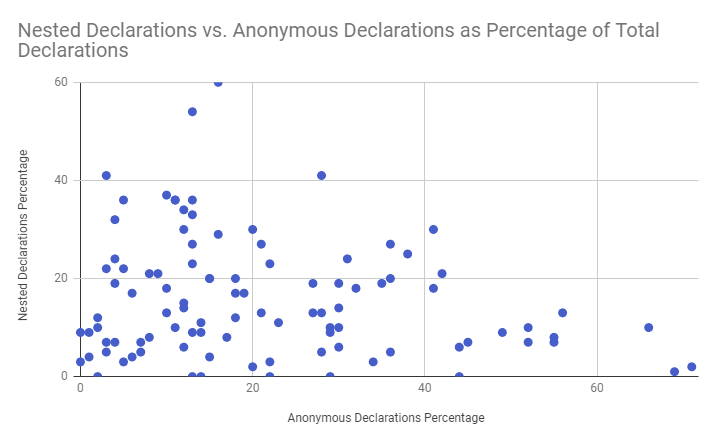
\includegraphics[width=0.8\textwidth]{NestedVsAnon.PNG}
    \caption{Comparing anonymous and local declaration occurences}
    \label{fig:NestedVsAnon}
  \end{center}
\end{figure}

There are 56 systems where the number of anonymous declarations are greater than nested declarations. There are 42 systems where the number of nested declarations exceed anonymous declarations. The chart below shows the relationship between these declarations.

There is a correlation coefficient of 0.19 across our dataset which indicates the use of anonymous or nested declarations are typically unrelated to each other.


\subsection{Usage Frequency of Anonymous, Local, and Nested Types}

\begin{figure}[H]
  \begin{center}
    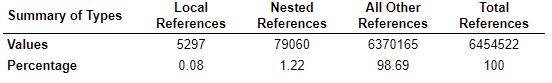
\includegraphics{References.PNG}
    \caption{Total type references across all 100 Java systems}
    \label{fig:References}
  \end{center}
\end{figure}

Our program could not track the references to anonymous classes. Since anonymous classes are used to declare and instantiate unnamed single children instances of a given class, anonymous classes cannot be referenced. We can only check the number of times the classes inherited by the anonymous class is referenced, either through its constructor when the anonymous class is declared, or through declaring variables that point to the anonymous class object. However due to the nature of anonymous classes, it can be assumed that each declaration of the anonymous class is used at least once after it is declared. Therefore we are assuming that anonymous declarations is equivalent to anonymous references which would give us an underestimate of 29085 anonymous references or 0.45\% of total references. Hence, we get a total anonymous, local, and nested references of 1.75\%. This number maybe miniscule but remember that it’s relative to every other references in the system, including pre-made libraries. Additionally, these types are not as common as other more “regular” types so it makes sense that they are not referenced as much as other types. Therefore, in terms of proportionality, a total reference count of 1.75\% for anonymous, local and nested references seem to be normal.

Next, is to consider the amount of declarations of anonymous, local and nested types compared to other declarations in the system. From our sample, we have 173751 declarations, where 16.74 \% are anonymous declarations, 0.51\% are local declarations, and 20.53\% are nested declarations, which amounts to 37.78\% of the total. But this number does not account for the systems with abnormally high amount of any of these types. Therefore, we need to total the average of each type. Where 19.57\% is the average anonymous declarations, 0.02\% is the average local declarations, and 14.92\% is the average nested declarations per system which totals to 34.51\%; only ~3\% off from the skewed total. From this, we can tell that anonymous, local, and nested declarations make up about a third of all the declarations in a system. This reinforces the fact that these types have niche uses but not as circumstantial as one might think. It also tells us that the outlier systems only skewed the data by 3\% which is maybe due to the low amount of outliers and their corresponding data not being too far off, for the most part.

\begin{figure}[H]
  \begin{center}
    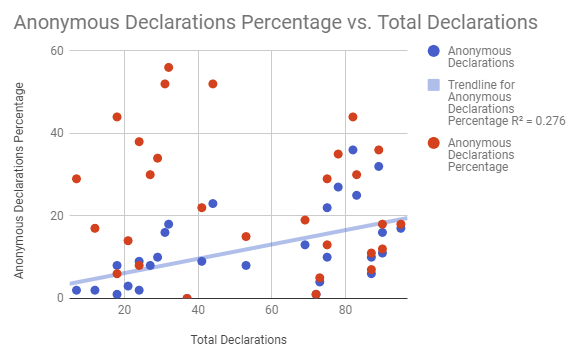
\includegraphics[width=0.8\textwidth]{AnonPercent.PNG}
    \caption{Anonymous declarations}
    \label{fig:AnonPercent}
  \end{center}
\end{figure}

In conclusion, anonymous, local and nested types make up a bigger part of the total declarations in a system, 34.51\%, than the total references in a system, 1.75\%. Both numbers seem to be consistent with the purpose of these types.

\subsection{Variability of Data from System to System}

Certain systems have more nested declarations than anonymous declarations and vice versa. A few systems also use local declarations to varying degrees. It appears that nested and anonymous types are declared almost all the time across all systems.

Analyzing the usage of local declarations, the data indicates that they are useful in specific cases but not widely used or declared. Out of the 31 systems that used local declarations, 16 were tools, the rest were frameworks, services, clients and libraries. One thing to note is that frameworks, services, clients and libraries do not need to use local declarations. There are a few of these systems that have no local declarations.

Concerning the use of nested and anonymous declarations, it appears that almost every type of system will make use of these declarations. However 42 systems had more nested declarations than anonymous declarations. Out of this selection: 22 were tools, the rest were libraries, clients and frameworks, or programs that depended on other systems. 61.29\% of systems that used local declarations also had more nested declarations than anonymous declarations. This seems to indicate that systems using more local declarations, tended to use more nested declarations as well. It appears that nested declarations are used more in frameworks than any other types of systems since they are the only type of system that consistently have more nested declarations than any other type.

As for the systems where anonymous declarations exceed nested declarations, out of the 57 only 12 used local declarations. So about 23.08\% of these systems used local declarations. This further supports the idea that Systems with nested declarations have more local declarations. As for the specific types of systems tending to have more anonymous declarations than nested ones, this does not show up in our sample.

The idea that specific types of systems requiring the use of a specific declaration is unfounded. We do not have conclusive evidence to support the claim. Not every database, library, service and framework used local declarations. This seems to indicate that local declarations are not a necessity for these systems, as roughly 50\% of these systems used local declarations and the others didn’t use them at all. Out of 52 Tool systems, only 16 used local declarations and 24 used more nested declarations than anonymous ones. The difference in usage could be a stylistic choice, rather than being a result of necessity.

\begin{figure}[H]
  \begin{center}
    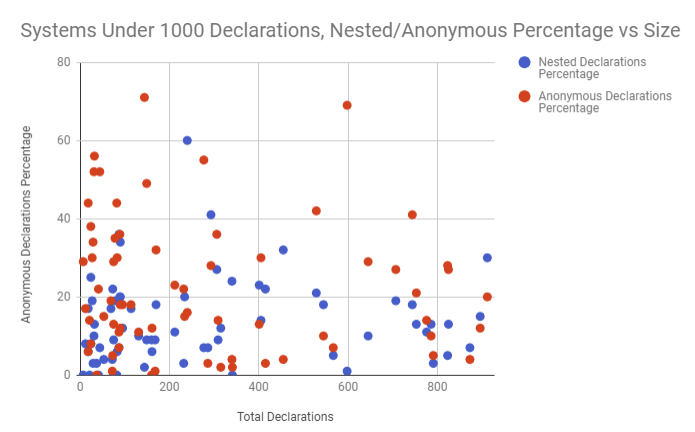
\includegraphics[width=0.8\textwidth]{Under1000.PNG}
    \caption{Comparing nested and anonymous declarations for smaller systems}
    \label{fig:Under1000}
  \end{center}
\end{figure}

\begin{figure}[H]
  \begin{center}
    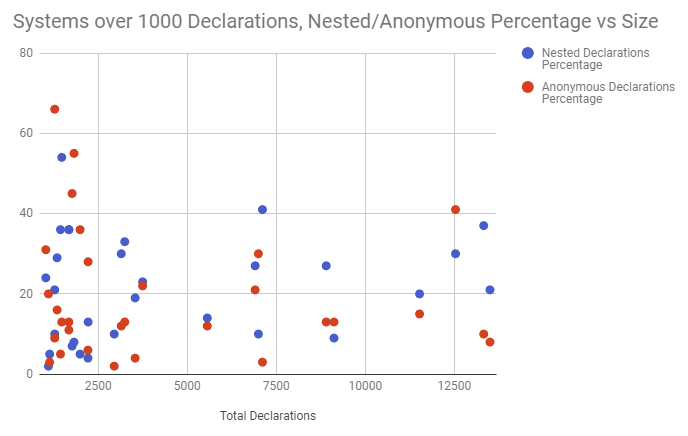
\includegraphics[width=0.8\textwidth]{Over1000.PNG}
    \caption{Comparing nested and anonymous declarations for larger systems}
    \label{fig:Over1000}
  \end{center}
\end{figure}

As for system size affecting the number of declarations, we have found no clear relationship between the two if we exclude the top 8 systems (by size). However when we look at the larger systems, we could say that as size increases, anonymous and nested declarations become less important compared to overall declarations, but it is quite weak. The ratio between the declaration types do not seem to be affected by system size.

In conclusion, the variability of certain declarations between systems based on the type of Systems might be due to stylistic choices rather than necessity. Of course there is always the possibility that certain declarations needed to be used, however the data we have gathered does not indicate that a specific type of system is dependant on a specific type of declaration. The data also suggests that system size has very little effect on these special declaration types.

\subsection{Sampling and Analyzing Process}


Selection of systems was broken out in a group effort where all team members selected 10 systems. In general most of the systems chosen were done so because they were featured prominently through GitHub searches in terms of popularity. In order for the sample to reflect the variety of java systems on GitHub, each member made sure to choose ten systems that did not necessarily belong to only one equivalence class of open source Java systems, but several. With regard to this variety, each member also made it a goal to select systems that were both large and relatively small. Checking the correlation between reported bugs and closed bugs in each system also played an important part in the selection process. Taking these sampling selection practices into account, the rather small sample size of 100 systems may be able to encompass the variations among all open source systems, albeit to a less than optimal degree due to the small sample.

In order to collect the information, a shared google sheets document was utilized and each member ran the analysis tool on the downloaded code, recording the output data. With regard to the analysis of said data, each system was given a general classification of its type (ie. tool, entertainment, service etc.). Analysts within the team then calculated the percentages of nested, local and anonymous declarations and references out of all declarations and references in the 100 systems. From these percentages, further analysis was performed concerning the relationship between anonymous and nested types, and the identification of outliers within the data.

\subsection{Possible Bugs in Our Analysis Tool}


Most of the bugs we encountered took the form of NullPointerExceptions, thrown by the node visitor. Usually, these exceptions were thrown when attempting to resolve the bindings of the nodes, which occurred for a number of different reasons: annotation nodes not creating bindings, and unsuccessful imports from external libraries, to name two. Thankfully, we were able to exploit the inherent design of Eclipse’s ASTs to circumvent these issues, by retrieving the qualified names for the unresolvable bindings from other nodes in the tree (usually child nodes). There is, of course, the very real possibility that our circumventions may have introduced other, less visible bugs into our software; however, we felt that data which may be slightly inaccurate is still more revealing than no data at all.

After each major change to our software, we made an effort to simultaneously rerun all of our analysis cases through the program again and re-record our new findings. Often there were no changes, apart from the filling in of data gaps which were caused by system crashes, but occasionally a few cells would increase or decrease slightly. As these periodic fluctuations always seemed to fit with our expectations of how the data should change, there is no immediate reason for us to believe that they were symptomatic of newly-introduced logical errors.

As an amusing aside, we did at one point encounter a NullPointerException which a bit of research revealed was caused by a bug in the Eclipse JDT itself. Recognizing immediately that any attempt at circumventing this issue would be a fool’s errand, we instead chose to simply swap out the code repository causing the crash for another.


\section{Discussion and Interpretation}

\subsection{Correctness of Results}

In so far that there is in fact a correct number of declarations and reference types for anonymous, local, and nested types in each Java system, if our results happened to match those counts it would most likely be by happenstance. This is mainly due to whatever notable bugs we have in our system, as well as the potential for unknown bugs that we are not even aware of. Noting this possibility, it is quite unlikely that our results do perfectly match what they should be, especially for the larger systems in which even small bugs can accumulate large inaccuraccies over time.

For the sake of assurance, we took whatever steps necessary to minimize these sources of error, given our timeframe and resources. We ran a number of controlled experiments involving smaller systems where we could generate expected values, and found that our results matched. While this was a useful exercise in checking for crash-inducing bugs and obvious logical missteps, there is ultimately still no guarantee that our calibrated software returns only correct results. However, we can believe that, in a sterile environment limited by our own coding abilities, the software does not tend to return glaringly incorrect results. As nothing has indicated to us that anyone else is capable of more certainty than that, we feel this is a sufficient degree of correctness. In terms of our program, while we may not know its output  is correct, we are reasonably confident that they are at least close to what they should be.

In terms of our data and sources, it seems that it can be a bit skewed. First, considering our programs were gathered from GitHub, most of them are classified as tools: 52\% while the rest fall under library: 19\%, framework: 5\%, service: 5\%, etc. This skewness maybe due to our broad definition of tool and the overall difficulty of classifying a system.But nonetheless, our data will inevitably revolve around analysis of tool systems. Conclusions about other category of systems will simply not have enough data to back it up.

Secondly, since we are basing the size of a system on its total number of declarations, most of our systems have less than 1000 declarations, 70\% to be exact. While the number of our “big” systems, the ones that have greater than 3000 declarations, are only at 12\%. And those systems can have declarations from around 4000 to 10000 plus. Thus, similar to our first problem, our analysis is skewed to systems with less than 1000 declarations. Otherwise, making conclusions about bigger systems will not have enough data to back it up.

In conclusion, our confidence lies in our program, while there is definitely room for improvement for our data. Due to our data, our analysis can only make viable conclusions about tool systems that are under 1000 declarations.

\subsection{Application to Other Java and non-Java Systems}

\subsubsection{Java Systems}

Given our selection of Java systems, we can be somewhat confident that the trends we have found can be generally representative of other Java systems. However, noting that we have a sample size of 100, which pales in comparison to the sheer number of actual open-source Java systems, let alone closed-source systems, we should be cautious not to overstep our bounds by making claims that are too strong.

For example, given that all our Java systems, except 1, have close to 0\% local declarations and references, we can reasonably infer that this trend may be present amongst other similar Java systems. While this is not a proclamation of certainty, a claim like this would be far more grounded than one claiming specific percentage uses of anonymous and nested declarations, which vary quite strongly across different systems. However, a far weaker claim, such as anonymous and nested types being utilized consistently across different systems of different types and sizes can be an indicator that these types would be used quite commonly in other systems.

Another indicator of how anonymous, local, and nested types would be different across Java systems, would be the age of the system, or more specifically, the Java version used in the system. As the Java language has developed over the years, more feature have been added, giving developers more options in how to solve problems. Take the introduction of lambda expressions in Java 8 for example. Prior to Java 8, some developers may have used anonymous Callable objects, which would contribute to anonymous declaration types for every Callable used. While there may still be developers averse to using lambda expressions, even working with systems using Java versions 8 and newer, the addition of lambda expressions would decrease anonymous declaration usage in each case they are used.


\subsubsection{Non-Java Systems}

For non-Java systems, making generalizations for anonymous, local, and nested types is split between being trivially easy, and being more difficult to make than for other Java-systems.

Non-Java systems that don’t support anonymous, local, or nested types, would evidently not use these respective types. Examples would include systems that operate under other programming paradigms such as Haskell, or Prolog. However, when these types are supported, answering this question can be difficult. In the absence of any tool to actually acquire empirical data on these type usages, we would have to resort to speculate on a number of fronts to make some roughly educated guess.

First, what type of non-Java systems are we analyzing, and do similar Java-equivalent systems exist? Independent of the language, if similar systems involve solving similar problems, and we are working with languages that provide similar tools, then in expectation developers may solve these problems in a similar manner. This mainly ties to the idea of design patterns being applicable across languages, but also with the use of nested, local, and anonymous classes.

Second, do other languages support features that allow developers to solve problems in a more appealing way than with anonymous, local and nested types. In this context, appealing could simply mean that statistically, developers opt to use these alternative means over anonymous, local and nested types given the availability for both? If such features do exist, we would expect that in aggregate, these types would appear less used proportionally than in their Java system equivalents. Inversely, does Java provide relevant features that detract from anonymous, local, and nested type usages that other languages do not? This would result in an opposite effect than the one mentioned before.

This is in no way an exhaustive list, as there are any number of factors that can impact how developers use anonymous, local, and nested types with varying languages.

\subsection{Practicality of Anonymous, Local, and Nested Types}

\subsubsection{How They Are Used in Theory}

Regarding the usability of nested, local, and anonymous types, according to Oracle, these types gives us the ability to put together the classes that are only used in one place. which increase the encapsulation and creates codes that are more concise, readable and easy to maintain. However, each of them is appropriate to use in specific situations. We can use local classes inside a block of code usually a method when we need to create more than one instance of a class. Anonymous classes are used to declare and instantiate a class simultaneously in a more concise manner than formally defining a class elsewhere and instantiating it once. This is typically done where the new class is only needed to be instantiated once, and  where the class’s extension from its parent class is not particularly lengthy.

\subsubsection{How They Are Used in Practice}

Based on the analysis conducted on the 100 open source systems, we found that local declarations are sparingly used, constituting only 37.75\% of all declarations. In particular, our analysis demonstrates that local types are substantially less common than nested and anonymous types. Given their rare occurrence in our chosen systems, it certainly doesn’t seem that much of the programming community considers local declaration types worthwhile. Furthermore, the number of bugs that we found while developing our software to count these types--though working with standard declarations was a comparative breeze--suggests that they are neglected as a usable construct.

However, the lack of usage of local types does not necessarily mean these declarations are useless. We might instead extrapolate from our findings that they simply serve a niche role, or are an unfamiliar concept to most programmers. These declarations are, after all, fairly uncommon outside of Java, and even then are a relatively new invention. Therefore, it could instead be more appropriate to say that the full extent of their usefulness has yet to be discovered, and at present the world of computer science has yet to catch up. As technology tends to progress in unpredictable ways, this statement is somewhat unfounded, but it may account better for the fact that programmers have evidently not outright rejected these modes of programming.

Alternatively, the minimal use of local types may not actually be a problem insofar that not all declaration types need to be popularly used. The fact that given features are rarely used does not mean that they useless but rather they fit a niche role designed to serve a specific set of problems. Even if local types continue to be ignored by the majority of Java programmers, it’s still there for those who need it for their purposes.

\subsubsection{Complications}

Regarding the extra complications that these types cause, from our experience it seems the complications are on counting these types with the ASTVisitor. Otherwise, to reiterate, the increased encapsulation should make the code easier to read and maintain. Although developers seem to frown upon local types as our data suggests. This maybe due to how local types work because they are usually defined within a method and most of the time when a programmer creates a method, most of that methods requirements are already made. So a local type seems like backwards implementation of a method for the most part. Local types also shares a lot of similar properties to nested types but without reusability of a nested type.

Depending on the type of nested class, there could be some limitations. Static nested classes do not have access to the methods and variables of their outer classes, and can only use them through object references. Meanwhile, inner classes do have access to these methods and variables since they are connected to an instance of the outer class, yet they cannot define static members. These rules could potentially cause frustration for Java programmers, but one could argue that the rules are only an extension of Java’s rules on scope and that these frustrated programmers must make the effort themselves to understand the implications and justifications for said rules. After all, nested classes as a construct are designed to create strong coupling between classes; so arises the need to carefully define the scopal relationships between these classes.

Overall, while anonymous, local and nested types have their own practical usage with the complications mostly dependent on the programmer’s skill, local types seem to perform a more niche job than the other types.

\subsection{Stability of Anonymous, Local, and Nested Types Across Versions}

Currently, our analysis tool is able to count type declarations and type references and distinguish them from nested, local, and anonymous types, so it already has the basic functionality to tackle this question. It is able to analyze multiple directories when given their paths, but this requires the user to manually download the system and feed the tool the path to each system. A possible addition could be the ability to pull multiple versions of a system when given a repository, eliminating the need for manual downloading and saving time. Another possible addition could be the automation of the collection of data into a spreadsheet. Our current tool outputs to the command line, so users have to manually record the data. The automation of this may save time and reduce the amount of error in the recording of data.

In terms of our analysis procedure, one of the largest changes would be to our sampling process of the Java systems. In addition to our original sampling process that is detailed previously, we would need to select systems that have multiple version releases. In a particular system we can analyze the changes in the number of the relevant types over minor version number updates and major version number updates. We can then derive trends for the system in regards to the relevant types and compare them to the trends in the other systems in our sample. Lastly, using a different code source other than github will likely help with the variety of systems to analyze.

\section{Conclusion}

In conclusion, the correctness of our results is not guaranteed. However, we have taken steps to ensure that our errors are minimized. We ran a number of controlled experiments involving smaller systems where we could generate expected values, and found that our results matched. This allowed us to test logical missteps and ensure no crashes would occur, but ultimately this does not guarantee the correctness of our result. The trends in the data seems to indicate that different types of systems do not depend on a specific declaration type. System sizes also do not seem to affect the ratio of the types declared, in relation to each other. The application of these declarations to non-Java systems are highly dependent on the similarity to Java. If the programming language does not support these declarations, there really is no point in speculation. However, if the language does support these declarations, there is a large amount of speculation to be made. This makes it quite difficult to predict how anonymous, nested and local declarations will be used. As for the usefulness of these types, anonymous and nested types are used in most of the sampled systems. However, with local types, there is no concrete conclusion on usefulness that we can draw from our data. The most we can say is that local types are seldomly used. Whether this is because they serve niche roles or the community has yet to discover the full extent of their capabilities, or simply because they are not practical is debatable. The fact that local types are used at all is indicative of its potential and cannot be discounted.

\section{Bibliography}
\begin{hangingpar}{2em}
  \item Anonymous Classes. (n.d.). Retrieved from Oracle, The Java Tutorials:\\ https://docs.oracle.com/javase/tutorial/java/javaOO/anonymousclasses.html
  \item Nested Classes. (n.d.). Retrieved from Oracle, The Java Tutorials:\\ https://docs.oracle.com/javase/tutorial/java/javaOO/nested.html
  \item Unit 18: Nested Classes. (n.d.). Retrieved from IBM, developerWorks:\\ https://www.ibm.com/developerworks/library/j-perry-nested-classes/index.html
  \item When to Use Nested Classes, Local Classes, Anonymous Classes and Lambda Expressions. (n.d.). Retrieved from Oracle, The Java Tutorials:\\ https://docs.oracle.com/javase/tutorial/java/javaOO/whentouse.html
\end{hangingpar}

\newpage

\section{Appendix}

\begin{figure}[h]
  \begin{center}
    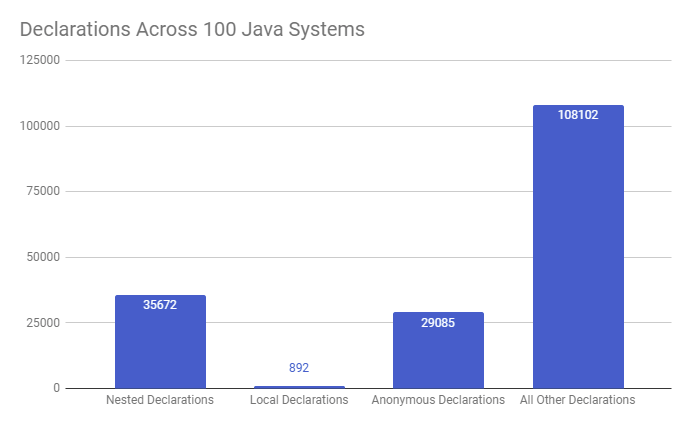
\includegraphics[width=0.7\textwidth]{DeclarationCount.PNG}
    \caption{Total type declaration counts across all 100 Java systems}
    \label{fig:DeclarationCount}
  \end{center}
\end{figure}

\begin{figure}[h]
  \begin{center}
    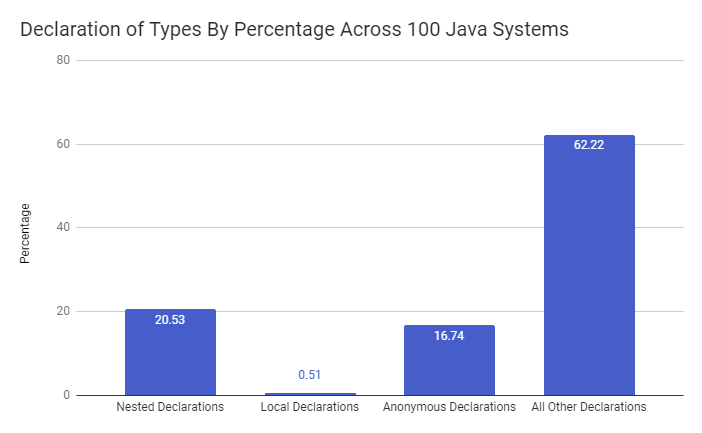
\includegraphics[width=0.7\textwidth]{DeclarationPercent.PNG}
    \caption{Total type declaration percentages across all 100 Java systems}
    \label{fig:DeclarationPercent}
  \end{center}
\end{figure}

\begin{figure}[h]
  \begin{center}
    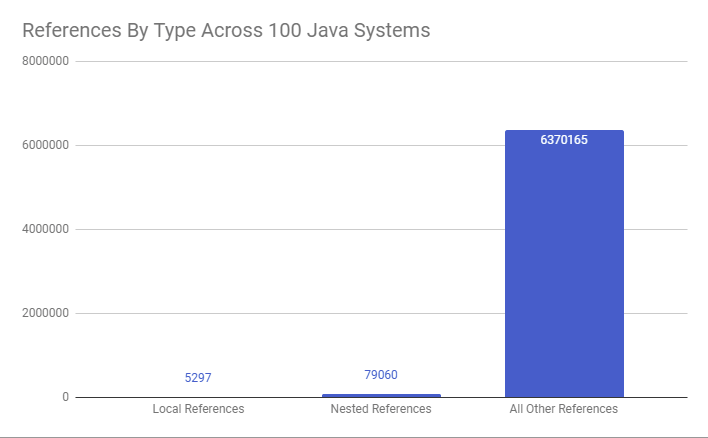
\includegraphics[width=0.7\textwidth]{ReferenceCount.PNG}
    \caption{Total type reference counts across all 100 Java systems}
    \label{fig:ReferenceCount}
  \end{center}
\end{figure}

\begin{figure}[h]
  \begin{center}
    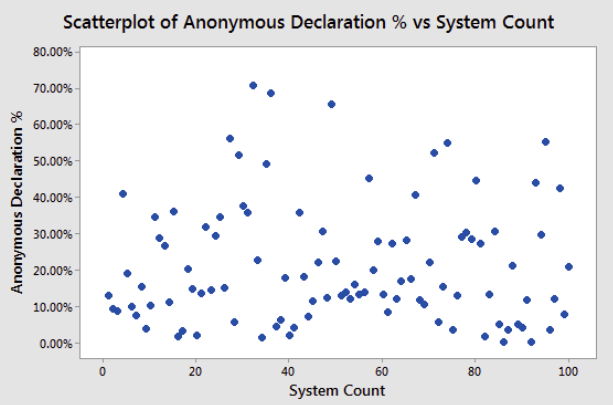
\includegraphics[width=0.7\textwidth]{AnonVsSystemDeclarations.PNG}
    \caption{Comparing anonymous and system declarations}
    \label{fig:AnonVsSystemDeclarations}
  \end{center}
\end{figure}

\begin{figure}[h]
  \begin{center}
    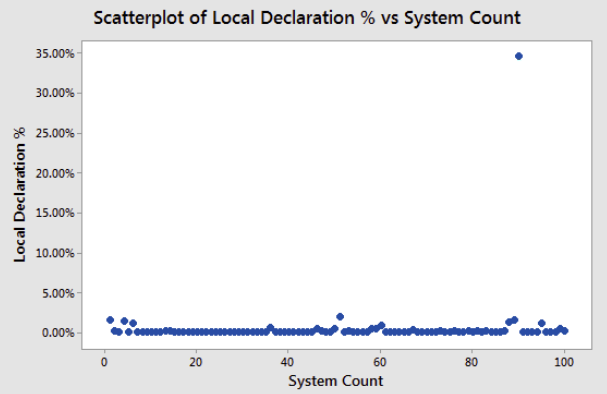
\includegraphics[width=0.7\textwidth]{LocalVsSystemDeclarations.PNG}
    \caption{Comparing local and system declarations}
    \label{fig:LocalVsSystemDeclarations}
  \end{center}
\end{figure}

\begin{figure}[h]
  \begin{center}
    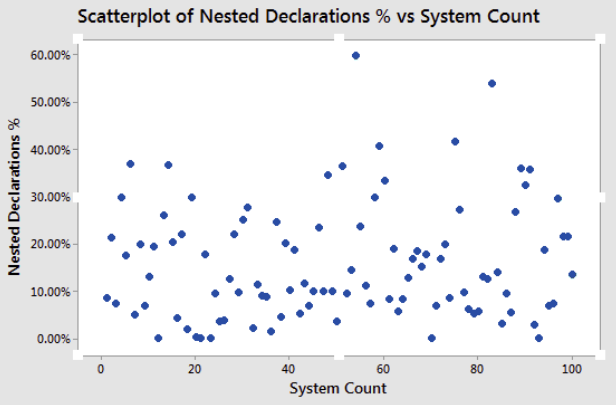
\includegraphics[width=0.7\textwidth]{NestedVsSystemDeclarations.PNG}
    \caption{Comparing nested and system declarations}
    \label{fig:NestedVsSystemDeclarations}
  \end{center}
\end{figure}

\end{document}
